\documentclass[twoside]{book}

% Packages required by doxygen
\usepackage{fixltx2e}
\usepackage{calc}
\usepackage{doxygen}
\usepackage[export]{adjustbox} % also loads graphicx
\usepackage{graphicx}
\usepackage[utf8]{inputenc}
\usepackage{makeidx}
\usepackage{multicol}
\usepackage{multirow}
\PassOptionsToPackage{warn}{textcomp}
\usepackage{textcomp}
\usepackage[nointegrals]{wasysym}
\usepackage[table]{xcolor}

% Font selection
\usepackage[T1]{fontenc}
\usepackage[scaled=.90]{helvet}
\usepackage{courier}
\usepackage{amssymb}
\usepackage{sectsty}
\renewcommand{\familydefault}{\sfdefault}
\allsectionsfont{%
  \fontseries{bc}\selectfont%
  \color{darkgray}%
}
\renewcommand{\DoxyLabelFont}{%
  \fontseries{bc}\selectfont%
  \color{darkgray}%
}
\newcommand{\+}{\discretionary{\mbox{\scriptsize$\hookleftarrow$}}{}{}}

% Page & text layout
\usepackage{geometry}
\geometry{%
  a4paper,%
  top=2.5cm,%
  bottom=2.5cm,%
  left=2.5cm,%
  right=2.5cm%
}
\tolerance=750
\hfuzz=15pt
\hbadness=750
\setlength{\emergencystretch}{15pt}
\setlength{\parindent}{0cm}
\setlength{\parskip}{3ex plus 2ex minus 2ex}
\makeatletter
\renewcommand{\paragraph}{%
  \@startsection{paragraph}{4}{0ex}{-1.0ex}{1.0ex}{%
    \normalfont\normalsize\bfseries\SS@parafont%
  }%
}
\renewcommand{\subparagraph}{%
  \@startsection{subparagraph}{5}{0ex}{-1.0ex}{1.0ex}{%
    \normalfont\normalsize\bfseries\SS@subparafont%
  }%
}
\makeatother

% Headers & footers
\usepackage{fancyhdr}
\pagestyle{fancyplain}
\fancyhead[LE]{\fancyplain{}{\bfseries\thepage}}
\fancyhead[CE]{\fancyplain{}{}}
\fancyhead[RE]{\fancyplain{}{\bfseries\leftmark}}
\fancyhead[LO]{\fancyplain{}{\bfseries\rightmark}}
\fancyhead[CO]{\fancyplain{}{}}
\fancyhead[RO]{\fancyplain{}{\bfseries\thepage}}
\fancyfoot[LE]{\fancyplain{}{}}
\fancyfoot[CE]{\fancyplain{}{}}
\fancyfoot[RE]{\fancyplain{}{\bfseries\scriptsize Generated by Doxygen }}
\fancyfoot[LO]{\fancyplain{}{\bfseries\scriptsize Generated by Doxygen }}
\fancyfoot[CO]{\fancyplain{}{}}
\fancyfoot[RO]{\fancyplain{}{}}
\renewcommand{\footrulewidth}{0.4pt}
\renewcommand{\chaptermark}[1]{%
  \markboth{#1}{}%
}
\renewcommand{\sectionmark}[1]{%
  \markright{\thesection\ #1}%
}

% Indices & bibliography
\usepackage{natbib}
\usepackage[titles]{tocloft}
\setcounter{tocdepth}{3}
\setcounter{secnumdepth}{5}
\makeindex

% Hyperlinks (required, but should be loaded last)
\usepackage{ifpdf}
\ifpdf
  \usepackage[pdftex,pagebackref=true]{hyperref}
\else
  \usepackage[ps2pdf,pagebackref=true]{hyperref}
\fi
\hypersetup{%
  colorlinks=true,%
  linkcolor=blue,%
  citecolor=blue,%
  unicode%
}

% Custom commands
\newcommand{\clearemptydoublepage}{%
  \newpage{\pagestyle{empty}\cleardoublepage}%
}

\usepackage{caption}
\captionsetup{labelsep=space,justification=centering,font={bf},singlelinecheck=off,skip=4pt,position=top}

%===== C O N T E N T S =====

\begin{document}

% Titlepage & ToC
\hypersetup{pageanchor=false,
             bookmarksnumbered=true,
             pdfencoding=unicode
            }
\pagenumbering{alph}
\begin{titlepage}
\vspace*{7cm}
\begin{center}%
{\Large Stack \\[1ex]\large 3.\+0 }\\
\vspace*{1cm}
{\large Generated by Doxygen 1.8.13}\\
\end{center}
\end{titlepage}
\clearemptydoublepage
\pagenumbering{roman}
\tableofcontents
\clearemptydoublepage
\pagenumbering{arabic}
\hypersetup{pageanchor=true}

%--- Begin generated contents ---
\chapter{Main Page}
\label{index}\hypertarget{index}{}Implements a stack class

\begin{DoxyVersion}{Version}
4.\+0
\end{DoxyVersion}
\begin{DoxyAuthor}{Author}
ShJ 
\end{DoxyAuthor}
\begin{DoxyDate}{Date}
05.\+03.\+2017 
\end{DoxyDate}

\chapter{Namespace Index}
\section{Namespace List}
Here is a list of all documented namespaces with brief descriptions\+:\begin{DoxyCompactList}
\item\contentsline{section}{\hyperlink{namespaceatom}{atom} \\*Common namespace }{\pageref{namespaceatom}}{}
\end{DoxyCompactList}

\chapter{Class Index}
\section{Class List}
Here are the classes, structs, unions and interfaces with brief descriptions\+:\begin{DoxyCompactList}
\item\contentsline{section}{\hyperlink{classstk_1_1stack__t}{stk\+::stack\+\_\+t$<$ Tp $>$} }{\pageref{classstk_1_1stack__t}}{}
\end{DoxyCompactList}

\chapter{File Index}
\section{File List}
Here is a list of all documented files with brief descriptions\+:\begin{DoxyCompactList}
\item\contentsline{section}{D\+:/\+Git\+Hub/\+Techno\+Atom/src/\hyperlink{debug__tools_8h}{debug\+\_\+tools.\+h} }{\pageref{debug__tools_8h}}{}
\item\contentsline{section}{D\+:/\+Git\+Hub/\+Techno\+Atom/src/\hyperlink{exceptions_8h}{exceptions.\+h} }{\pageref{exceptions_8h}}{}
\item\contentsline{section}{D\+:/\+Git\+Hub/\+Techno\+Atom/src/array/\hyperlink{array_8h}{array.\+h} }{\pageref{array_8h}}{}
\item\contentsline{section}{D\+:/\+Git\+Hub/\+Techno\+Atom/src/array/implement/{\bfseries array.\+hpp} }{\pageref{array_8hpp}}{}
\item\contentsline{section}{D\+:/\+Git\+Hub/\+Techno\+Atom/src/stack/\hyperlink{stack_8h}{stack.\+h} }{\pageref{stack_8h}}{}
\item\contentsline{section}{D\+:/\+Git\+Hub/\+Techno\+Atom/src/stack/implement/{\bfseries stack.\+hpp} }{\pageref{stack_8hpp}}{}
\item\contentsline{section}{D\+:/\+Git\+Hub/\+Techno\+Atom/src/vector/\hyperlink{vector_8h}{vector.\+h} }{\pageref{vector_8h}}{}
\item\contentsline{section}{D\+:/\+Git\+Hub/\+Techno\+Atom/src/vector/implement/{\bfseries vector.\+hpp} }{\pageref{vector_8hpp}}{}
\end{DoxyCompactList}

\chapter{Namespace Documentation}
\hypertarget{namespacestk}{}\section{stk Namespace Reference}
\label{namespacestk}\index{stk@{stk}}


There the stack class describes.  


\subsection*{Classes}
\begin{DoxyCompactItemize}
\item 
class \hyperlink{classstk_1_1stack__t}{stack\+\_\+t}
\end{DoxyCompactItemize}


\subsection{Detailed Description}
There the stack class describes. 
\chapter{Class Documentation}
\hypertarget{classstk_1_1stack__t}{}\section{stk\+:\+:stack\+\_\+t$<$ Tp $>$ Class Template Reference}
\label{classstk_1_1stack__t}\index{stk\+::stack\+\_\+t$<$ Tp $>$@{stk\+::stack\+\_\+t$<$ Tp $>$}}


{\ttfamily \#include $<$stack.\+h$>$}



Collaboration diagram for stk\+:\+:stack\+\_\+t$<$ Tp $>$\+:
\nopagebreak
\begin{figure}[H]
\begin{center}
\leavevmode
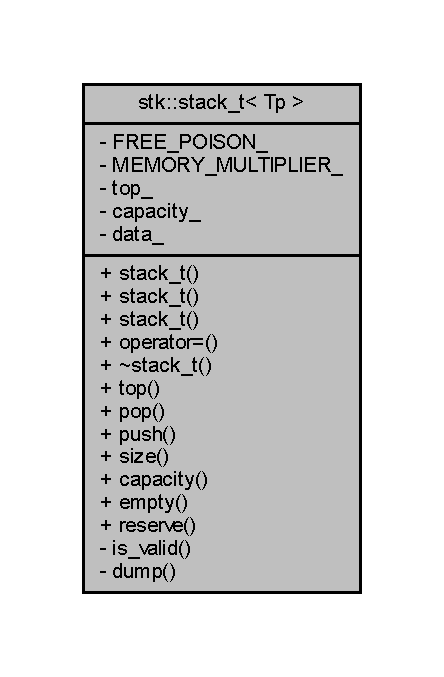
\includegraphics[width=213pt]{classstk_1_1stack__t__coll__graph}
\end{center}
\end{figure}
\subsection*{Public Types}
\begin{DoxyCompactItemize}
\item 
\mbox{\Hypertarget{classstk_1_1stack__t_a2e10db77beb285902df2b32f30209067}\label{classstk_1_1stack__t_a2e10db77beb285902df2b32f30209067}} 
using \hyperlink{classstk_1_1stack__t_a2e10db77beb285902df2b32f30209067}{value\+\_\+type} = Tp
\begin{DoxyCompactList}\small\item\em Element type. \end{DoxyCompactList}\item 
\mbox{\Hypertarget{classstk_1_1stack__t_a0beb74f603c2354cb9af98ee65801ce7}\label{classstk_1_1stack__t_a0beb74f603c2354cb9af98ee65801ce7}} 
using \hyperlink{classstk_1_1stack__t_a0beb74f603c2354cb9af98ee65801ce7}{const\+\_\+value\+\_\+type} = const Tp
\begin{DoxyCompactList}\small\item\em Const element type. \end{DoxyCompactList}\item 
\mbox{\Hypertarget{classstk_1_1stack__t_a591d5ffc540c9f27e5618f9aa4d67cad}\label{classstk_1_1stack__t_a591d5ffc540c9f27e5618f9aa4d67cad}} 
using \hyperlink{classstk_1_1stack__t_a591d5ffc540c9f27e5618f9aa4d67cad}{size\+\_\+type} = std\+::size\+\_\+t
\begin{DoxyCompactList}\small\item\em Size type. \end{DoxyCompactList}\end{DoxyCompactItemize}
\subsection*{Public Member Functions}
\begin{DoxyCompactItemize}
\item 
\mbox{\Hypertarget{classstk_1_1stack__t_ad8f2c6c72f3cc6d0b55c37c18ba77935}\label{classstk_1_1stack__t_ad8f2c6c72f3cc6d0b55c37c18ba77935}} 
\hyperlink{classstk_1_1stack__t_ad8f2c6c72f3cc6d0b55c37c18ba77935}{stack\+\_\+t} ()
\begin{DoxyCompactList}\small\item\em Default constructor. \end{DoxyCompactList}\item 
\hyperlink{classstk_1_1stack__t_acf68532e10f96d64c7745372dd1afba2}{stack\+\_\+t} (const \hyperlink{classstk_1_1stack__t_a591d5ffc540c9f27e5618f9aa4d67cad}{size\+\_\+type} n)
\item 
\hyperlink{classstk_1_1stack__t_ac5b1b45543c317bead3fe05ba64618ae}{stack\+\_\+t} (const \hyperlink{classstk_1_1stack__t}{stack\+\_\+t} \&stack)
\item 
\hyperlink{classstk_1_1stack__t}{stack\+\_\+t} \& \hyperlink{classstk_1_1stack__t_ae89dec429ddba4dda06f6c57fc688cc9}{operator=} (const \hyperlink{classstk_1_1stack__t}{stack\+\_\+t} \&stack)
\item 
\hyperlink{classstk_1_1stack__t_a45e9376d38de6b4c43c0edd54138edaa}{$\sim$stack\+\_\+t} ()
\item 
\hyperlink{classstk_1_1stack__t_a2e10db77beb285902df2b32f30209067}{value\+\_\+type} \hyperlink{classstk_1_1stack__t_a8850aa2ebf5ab0be43549a49b4d24339}{top} () const
\item 
void \hyperlink{classstk_1_1stack__t_a498151ba872e2b9ae2f9326b80efbbd3}{pop} ()
\item 
void \hyperlink{classstk_1_1stack__t_a17e043f3eb3b4ae3b0494a4e0ff1a1b5}{push} (\hyperlink{classstk_1_1stack__t_a0beb74f603c2354cb9af98ee65801ce7}{const\+\_\+value\+\_\+type} \&x)
\item 
\hyperlink{classstk_1_1stack__t_a591d5ffc540c9f27e5618f9aa4d67cad}{size\+\_\+type} \hyperlink{classstk_1_1stack__t_a3770048637478cc005d11a47ee4df148}{size} () const
\item 
\hyperlink{classstk_1_1stack__t_a591d5ffc540c9f27e5618f9aa4d67cad}{size\+\_\+type} \hyperlink{classstk_1_1stack__t_a04b3af82e2cf60df75bf3b8507c5de9a}{capacity} () const
\item 
bool \hyperlink{classstk_1_1stack__t_ab4878c2c4a3b11d35b67323a0f473813}{empty} () const
\item 
bool \hyperlink{classstk_1_1stack__t_a4bbfc186d4b0eab296b620b72d8f872d}{reserve} (const \hyperlink{classstk_1_1stack__t_a591d5ffc540c9f27e5618f9aa4d67cad}{size\+\_\+type} n)
\end{DoxyCompactItemize}
\subsection*{Private Member Functions}
\begin{DoxyCompactItemize}
\item 
bool \hyperlink{classstk_1_1stack__t_a981df1d2676a6253d943c8b42db6e8f0}{is\+\_\+valid} () const
\item 
void \hyperlink{classstk_1_1stack__t_a5b880836e779c81052eb82e7f435ab54}{dump} (const char $\ast$function\+\_\+name) const
\end{DoxyCompactItemize}
\subsection*{Private Attributes}
\begin{DoxyCompactItemize}
\item 
\mbox{\Hypertarget{classstk_1_1stack__t_aeaff281674605712b238b9d482b0d395}\label{classstk_1_1stack__t_aeaff281674605712b238b9d482b0d395}} 
\hyperlink{classstk_1_1stack__t_a0beb74f603c2354cb9af98ee65801ce7}{const\+\_\+value\+\_\+type} \hyperlink{classstk_1_1stack__t_aeaff281674605712b238b9d482b0d395}{F\+R\+E\+E\+\_\+\+P\+O\+I\+S\+O\+N\+\_\+} = \hyperlink{classstk_1_1stack__t_a2e10db77beb285902df2b32f30209067}{value\+\_\+type}()
\begin{DoxyCompactList}\small\item\em Constant for mark the empty fields. \end{DoxyCompactList}\item 
\mbox{\Hypertarget{classstk_1_1stack__t_a72607554a016dbb0e6b5cc92accdce03}\label{classstk_1_1stack__t_a72607554a016dbb0e6b5cc92accdce03}} 
const \hyperlink{classstk_1_1stack__t_a591d5ffc540c9f27e5618f9aa4d67cad}{size\+\_\+type} \hyperlink{classstk_1_1stack__t_a72607554a016dbb0e6b5cc92accdce03}{M\+E\+M\+O\+R\+Y\+\_\+\+M\+U\+L\+T\+I\+P\+L\+I\+E\+R\+\_\+} = 2u
\begin{DoxyCompactList}\small\item\em Constant memory increase. \end{DoxyCompactList}\item 
\mbox{\Hypertarget{classstk_1_1stack__t_aa26173e9f9fe76e7e28ca71b1e17c9ef}\label{classstk_1_1stack__t_aa26173e9f9fe76e7e28ca71b1e17c9ef}} 
\hyperlink{classstk_1_1stack__t_a591d5ffc540c9f27e5618f9aa4d67cad}{size\+\_\+type} \hyperlink{classstk_1_1stack__t_aa26173e9f9fe76e7e28ca71b1e17c9ef}{top\+\_\+}
\begin{DoxyCompactList}\small\item\em Pointer on the top item of the stack. \end{DoxyCompactList}\item 
\mbox{\Hypertarget{classstk_1_1stack__t_ace387ef68b512dd54537f2c8ebe3d0d5}\label{classstk_1_1stack__t_ace387ef68b512dd54537f2c8ebe3d0d5}} 
\hyperlink{classstk_1_1stack__t_a591d5ffc540c9f27e5618f9aa4d67cad}{size\+\_\+type} \hyperlink{classstk_1_1stack__t_ace387ef68b512dd54537f2c8ebe3d0d5}{capacity\+\_\+}
\begin{DoxyCompactList}\small\item\em Capacity of the stack. \end{DoxyCompactList}\item 
\mbox{\Hypertarget{classstk_1_1stack__t_a828b3c97415c648a9155e4f643d2ccb9}\label{classstk_1_1stack__t_a828b3c97415c648a9155e4f643d2ccb9}} 
\hyperlink{classstk_1_1stack__t_a2e10db77beb285902df2b32f30209067}{value\+\_\+type} $\ast$ \hyperlink{classstk_1_1stack__t_a828b3c97415c648a9155e4f643d2ccb9}{data\+\_\+}
\begin{DoxyCompactList}\small\item\em Stack base on dynamic array. \end{DoxyCompactList}\end{DoxyCompactItemize}


\subsection{Detailed Description}
\subsubsection*{template$<$typename Tp = int$>$\newline
class stk\+::stack\+\_\+t$<$ Tp $>$}


\begin{DoxyTemplParams}{Template Parameters}
{\em Tp} & The type of the value in the stack (the default type is int) \\
\hline
\end{DoxyTemplParams}


\subsection{Constructor \& Destructor Documentation}
\mbox{\Hypertarget{classstk_1_1stack__t_acf68532e10f96d64c7745372dd1afba2}\label{classstk_1_1stack__t_acf68532e10f96d64c7745372dd1afba2}} 
\index{stk\+::stack\+\_\+t@{stk\+::stack\+\_\+t}!stack\+\_\+t@{stack\+\_\+t}}
\index{stack\+\_\+t@{stack\+\_\+t}!stk\+::stack\+\_\+t@{stk\+::stack\+\_\+t}}
\subsubsection{\texorpdfstring{stack\+\_\+t()}{stack\_t()}\hspace{0.1cm}{\footnotesize\ttfamily [1/2]}}
{\footnotesize\ttfamily template$<$typename Tp $>$ \\
\hyperlink{classstk_1_1stack__t}{stk\+::stack\+\_\+t}$<$ Tp $>$\+::\hyperlink{classstk_1_1stack__t}{stack\+\_\+t} (\begin{DoxyParamCaption}\item[{const \hyperlink{classstk_1_1stack__t_a591d5ffc540c9f27e5618f9aa4d67cad}{size\+\_\+type}}]{n }\end{DoxyParamCaption})\hspace{0.3cm}{\ttfamily [explicit]}}

Constructor Reserve memory to n elements 
\begin{DoxyParams}{Parameters}
{\em n} & The number of elements for which memory is allocated \\
\hline
\end{DoxyParams}
\mbox{\Hypertarget{classstk_1_1stack__t_ac5b1b45543c317bead3fe05ba64618ae}\label{classstk_1_1stack__t_ac5b1b45543c317bead3fe05ba64618ae}} 
\index{stk\+::stack\+\_\+t@{stk\+::stack\+\_\+t}!stack\+\_\+t@{stack\+\_\+t}}
\index{stack\+\_\+t@{stack\+\_\+t}!stk\+::stack\+\_\+t@{stk\+::stack\+\_\+t}}
\subsubsection{\texorpdfstring{stack\+\_\+t()}{stack\_t()}\hspace{0.1cm}{\footnotesize\ttfamily [2/2]}}
{\footnotesize\ttfamily template$<$typename Tp $>$ \\
\hyperlink{classstk_1_1stack__t}{stk\+::stack\+\_\+t}$<$ Tp $>$\+::\hyperlink{classstk_1_1stack__t}{stack\+\_\+t} (\begin{DoxyParamCaption}\item[{const \hyperlink{classstk_1_1stack__t}{stack\+\_\+t}$<$ Tp $>$ \&}]{stack }\end{DoxyParamCaption})}

The copy constructor 
\begin{DoxyParams}{Parameters}
{\em stack} & The copy source \\
\hline
\end{DoxyParams}
\mbox{\Hypertarget{classstk_1_1stack__t_a45e9376d38de6b4c43c0edd54138edaa}\label{classstk_1_1stack__t_a45e9376d38de6b4c43c0edd54138edaa}} 
\index{stk\+::stack\+\_\+t@{stk\+::stack\+\_\+t}!````~stack\+\_\+t@{$\sim$stack\+\_\+t}}
\index{````~stack\+\_\+t@{$\sim$stack\+\_\+t}!stk\+::stack\+\_\+t@{stk\+::stack\+\_\+t}}
\subsubsection{\texorpdfstring{$\sim$stack\+\_\+t()}{~stack\_t()}}
{\footnotesize\ttfamily template$<$typename Tp = int$>$ \\
\hyperlink{classstk_1_1stack__t}{stk\+::stack\+\_\+t}$<$ Tp $>$\+::$\sim$\hyperlink{classstk_1_1stack__t}{stack\+\_\+t} (\begin{DoxyParamCaption}{ }\end{DoxyParamCaption})\hspace{0.3cm}{\ttfamily [inline]}}

Destructor Removes allocated memory 

\subsection{Member Function Documentation}
\mbox{\Hypertarget{classstk_1_1stack__t_a04b3af82e2cf60df75bf3b8507c5de9a}\label{classstk_1_1stack__t_a04b3af82e2cf60df75bf3b8507c5de9a}} 
\index{stk\+::stack\+\_\+t@{stk\+::stack\+\_\+t}!capacity@{capacity}}
\index{capacity@{capacity}!stk\+::stack\+\_\+t@{stk\+::stack\+\_\+t}}
\subsubsection{\texorpdfstring{capacity()}{capacity()}}
{\footnotesize\ttfamily template$<$typename Tp = int$>$ \\
\hyperlink{classstk_1_1stack__t_a591d5ffc540c9f27e5618f9aa4d67cad}{size\+\_\+type} \hyperlink{classstk_1_1stack__t}{stk\+::stack\+\_\+t}$<$ Tp $>$\+::capacity (\begin{DoxyParamCaption}{ }\end{DoxyParamCaption}) const\hspace{0.3cm}{\ttfamily [inline]}}

Capacity \begin{DoxyReturn}{Returns}
Capacity of the stack 
\end{DoxyReturn}
\mbox{\Hypertarget{classstk_1_1stack__t_a5b880836e779c81052eb82e7f435ab54}\label{classstk_1_1stack__t_a5b880836e779c81052eb82e7f435ab54}} 
\index{stk\+::stack\+\_\+t@{stk\+::stack\+\_\+t}!dump@{dump}}
\index{dump@{dump}!stk\+::stack\+\_\+t@{stk\+::stack\+\_\+t}}
\subsubsection{\texorpdfstring{dump()}{dump()}}
{\footnotesize\ttfamily template$<$typename Tp $>$ \\
void \hyperlink{classstk_1_1stack__t}{stk\+::stack\+\_\+t}$<$ Tp $>$\+::dump (\begin{DoxyParamCaption}\item[{const char $\ast$}]{function\+\_\+name }\end{DoxyParamCaption}) const\hspace{0.3cm}{\ttfamily [private]}}

Dumper Create file \char`\"{}\+\_\+\+\_\+stack\+\_\+dump.\+txt\char`\"{} where is information about stack\textquotesingle{}s status 
\begin{DoxyParams}{Parameters}
{\em function\+\_\+name} & Name of function which call this method \\
\hline
\end{DoxyParams}
\mbox{\Hypertarget{classstk_1_1stack__t_ab4878c2c4a3b11d35b67323a0f473813}\label{classstk_1_1stack__t_ab4878c2c4a3b11d35b67323a0f473813}} 
\index{stk\+::stack\+\_\+t@{stk\+::stack\+\_\+t}!empty@{empty}}
\index{empty@{empty}!stk\+::stack\+\_\+t@{stk\+::stack\+\_\+t}}
\subsubsection{\texorpdfstring{empty()}{empty()}}
{\footnotesize\ttfamily template$<$typename Tp = int$>$ \\
bool \hyperlink{classstk_1_1stack__t}{stk\+::stack\+\_\+t}$<$ Tp $>$\+::empty (\begin{DoxyParamCaption}{ }\end{DoxyParamCaption}) const\hspace{0.3cm}{\ttfamily [inline]}}

Checks the emptiness of the stack 
\begin{DoxyExceptions}{Exceptions}
{\em std\+::exception} & From \hyperlink{stack_8h_a4ad7af85cae2910ffcf6bfbcb8278886}{A\+S\+S\+E\+R\+T\+\_\+\+V\+A\+L\+I\+D()} when stack is not valid \\
\hline
\end{DoxyExceptions}
\begin{DoxyReturn}{Returns}
True if stack is empty, otherwise false 
\end{DoxyReturn}
\mbox{\Hypertarget{classstk_1_1stack__t_a981df1d2676a6253d943c8b42db6e8f0}\label{classstk_1_1stack__t_a981df1d2676a6253d943c8b42db6e8f0}} 
\index{stk\+::stack\+\_\+t@{stk\+::stack\+\_\+t}!is\+\_\+valid@{is\+\_\+valid}}
\index{is\+\_\+valid@{is\+\_\+valid}!stk\+::stack\+\_\+t@{stk\+::stack\+\_\+t}}
\subsubsection{\texorpdfstring{is\+\_\+valid()}{is\_valid()}}
{\footnotesize\ttfamily template$<$typename Tp $>$ \\
bool \hyperlink{classstk_1_1stack__t}{stk\+::stack\+\_\+t}$<$ Tp $>$\+::is\+\_\+valid (\begin{DoxyParamCaption}{ }\end{DoxyParamCaption}) const\hspace{0.3cm}{\ttfamily [private]}}

Silent verifier \begin{DoxyReturn}{Returns}
True if stack is valid else return false 
\end{DoxyReturn}
\mbox{\Hypertarget{classstk_1_1stack__t_ae89dec429ddba4dda06f6c57fc688cc9}\label{classstk_1_1stack__t_ae89dec429ddba4dda06f6c57fc688cc9}} 
\index{stk\+::stack\+\_\+t@{stk\+::stack\+\_\+t}!operator=@{operator=}}
\index{operator=@{operator=}!stk\+::stack\+\_\+t@{stk\+::stack\+\_\+t}}
\subsubsection{\texorpdfstring{operator=()}{operator=()}}
{\footnotesize\ttfamily template$<$typename Tp $>$ \\
\hyperlink{classstk_1_1stack__t}{stack\+\_\+t}$<$ Tp $>$ \& \hyperlink{classstk_1_1stack__t}{stk\+::stack\+\_\+t}$<$ Tp $>$\+::operator= (\begin{DoxyParamCaption}\item[{const \hyperlink{classstk_1_1stack__t}{stack\+\_\+t}$<$ Tp $>$ \&}]{stack }\end{DoxyParamCaption})}

The assignment operator 
\begin{DoxyParams}{Parameters}
{\em stack} & The source of the assignment \\
\hline
\end{DoxyParams}
\begin{DoxyReturn}{Returns}
Reference to the calling object 
\end{DoxyReturn}
\mbox{\Hypertarget{classstk_1_1stack__t_a498151ba872e2b9ae2f9326b80efbbd3}\label{classstk_1_1stack__t_a498151ba872e2b9ae2f9326b80efbbd3}} 
\index{stk\+::stack\+\_\+t@{stk\+::stack\+\_\+t}!pop@{pop}}
\index{pop@{pop}!stk\+::stack\+\_\+t@{stk\+::stack\+\_\+t}}
\subsubsection{\texorpdfstring{pop()}{pop()}}
{\footnotesize\ttfamily template$<$typename Tp $>$ \\
void \hyperlink{classstk_1_1stack__t}{stk\+::stack\+\_\+t}$<$ Tp $>$\+::pop (\begin{DoxyParamCaption}{ }\end{DoxyParamCaption})}

Delete the item from the stack 
\begin{DoxyExceptions}{Exceptions}
{\em std\+::exception} & From \hyperlink{stack_8h_a4ad7af85cae2910ffcf6bfbcb8278886}{A\+S\+S\+E\+R\+T\+\_\+\+V\+A\+L\+I\+D()} when stack is not valid \\
\hline
{\em std\+::out\+\_\+of\+\_\+range} & When stack is empty \\
\hline
\end{DoxyExceptions}
\mbox{\Hypertarget{classstk_1_1stack__t_a17e043f3eb3b4ae3b0494a4e0ff1a1b5}\label{classstk_1_1stack__t_a17e043f3eb3b4ae3b0494a4e0ff1a1b5}} 
\index{stk\+::stack\+\_\+t@{stk\+::stack\+\_\+t}!push@{push}}
\index{push@{push}!stk\+::stack\+\_\+t@{stk\+::stack\+\_\+t}}
\subsubsection{\texorpdfstring{push()}{push()}}
{\footnotesize\ttfamily template$<$typename Tp $>$ \\
void \hyperlink{classstk_1_1stack__t}{stk\+::stack\+\_\+t}$<$ Tp $>$\+::push (\begin{DoxyParamCaption}\item[{\hyperlink{classstk_1_1stack__t_a0beb74f603c2354cb9af98ee65801ce7}{const\+\_\+value\+\_\+type} \&}]{x }\end{DoxyParamCaption})}

Append new item in the stack 
\begin{DoxyParams}{Parameters}
{\em x} & The element that will be added to the stack \\
\hline
\end{DoxyParams}

\begin{DoxyExceptions}{Exceptions}
{\em std\+::exception} & From \hyperlink{stack_8h_a4ad7af85cae2910ffcf6bfbcb8278886}{A\+S\+S\+E\+R\+T\+\_\+\+V\+A\+L\+I\+D()} when stack is not valid \\
\hline
{\em std\+::bad\+\_\+alloc} & When the memory is not allocated \\
\hline
\end{DoxyExceptions}
\mbox{\Hypertarget{classstk_1_1stack__t_a4bbfc186d4b0eab296b620b72d8f872d}\label{classstk_1_1stack__t_a4bbfc186d4b0eab296b620b72d8f872d}} 
\index{stk\+::stack\+\_\+t@{stk\+::stack\+\_\+t}!reserve@{reserve}}
\index{reserve@{reserve}!stk\+::stack\+\_\+t@{stk\+::stack\+\_\+t}}
\subsubsection{\texorpdfstring{reserve()}{reserve()}}
{\footnotesize\ttfamily template$<$typename Tp $>$ \\
bool \hyperlink{classstk_1_1stack__t}{stk\+::stack\+\_\+t}$<$ Tp $>$\+::reserve (\begin{DoxyParamCaption}\item[{const \hyperlink{classstk_1_1stack__t_a591d5ffc540c9f27e5618f9aa4d67cad}{size\+\_\+type}}]{n }\end{DoxyParamCaption})}

Reserve a memory 
\begin{DoxyParams}{Parameters}
{\em n} & The number of elements for which memory is allocated \\
\hline
\end{DoxyParams}
\begin{DoxyReturn}{Returns}
True if memory allocated, otherwise false 
\end{DoxyReturn}
\mbox{\Hypertarget{classstk_1_1stack__t_a3770048637478cc005d11a47ee4df148}\label{classstk_1_1stack__t_a3770048637478cc005d11a47ee4df148}} 
\index{stk\+::stack\+\_\+t@{stk\+::stack\+\_\+t}!size@{size}}
\index{size@{size}!stk\+::stack\+\_\+t@{stk\+::stack\+\_\+t}}
\subsubsection{\texorpdfstring{size()}{size()}}
{\footnotesize\ttfamily template$<$typename Tp = int$>$ \\
\hyperlink{classstk_1_1stack__t_a591d5ffc540c9f27e5618f9aa4d67cad}{size\+\_\+type} \hyperlink{classstk_1_1stack__t}{stk\+::stack\+\_\+t}$<$ Tp $>$\+::size (\begin{DoxyParamCaption}{ }\end{DoxyParamCaption}) const\hspace{0.3cm}{\ttfamily [inline]}}

Currently size of the stack \begin{DoxyReturn}{Returns}
Count of the item in the stack 
\end{DoxyReturn}
\mbox{\Hypertarget{classstk_1_1stack__t_a8850aa2ebf5ab0be43549a49b4d24339}\label{classstk_1_1stack__t_a8850aa2ebf5ab0be43549a49b4d24339}} 
\index{stk\+::stack\+\_\+t@{stk\+::stack\+\_\+t}!top@{top}}
\index{top@{top}!stk\+::stack\+\_\+t@{stk\+::stack\+\_\+t}}
\subsubsection{\texorpdfstring{top()}{top()}}
{\footnotesize\ttfamily template$<$typename Tp $>$ \\
Tp \hyperlink{classstk_1_1stack__t}{stk\+::stack\+\_\+t}$<$ Tp $>$\+::top (\begin{DoxyParamCaption}{ }\end{DoxyParamCaption}) const}

Get the item from the stack 
\begin{DoxyExceptions}{Exceptions}
{\em std\+::exception} & From \hyperlink{stack_8h_a4ad7af85cae2910ffcf6bfbcb8278886}{A\+S\+S\+E\+R\+T\+\_\+\+V\+A\+L\+I\+D()} when stack is not valid \\
\hline
\end{DoxyExceptions}
\begin{DoxyReturn}{Returns}
The top item from the stack 
\end{DoxyReturn}


The documentation for this class was generated from the following file\+:\begin{DoxyCompactItemize}
\item 
D\+:/\+Git\+Hub/\+Techno\+Atom/stack/\hyperlink{stack_8h}{stack.\+h}\end{DoxyCompactItemize}

\chapter{File Documentation}
\hypertarget{stack_8h}{}\section{D\+:/\+Git\+Hub/\+Techno\+Atom/stack/stack.h File Reference}
\label{stack_8h}\index{D\+:/\+Git\+Hub/\+Techno\+Atom/stack/stack.\+h@{D\+:/\+Git\+Hub/\+Techno\+Atom/stack/stack.\+h}}
{\ttfamily \#include $<$stdexcept$>$}\newline
{\ttfamily \#include $<$cassert$>$}\newline
{\ttfamily \#include $<$fstream$>$}\newline
{\ttfamily \#include $<$ctime$>$}\newline
{\ttfamily \#include $<$algorithm$>$}\newline
\subsection*{Classes}
\begin{DoxyCompactItemize}
\item 
class \hyperlink{classstk_1_1stack__t}{stk\+::stack\+\_\+t$<$ Tp $>$}
\end{DoxyCompactItemize}
\subsection*{Namespaces}
\begin{DoxyCompactItemize}
\item 
 \hyperlink{namespacestk}{stk}
\begin{DoxyCompactList}\small\item\em There the stack class describes. \end{DoxyCompactList}\end{DoxyCompactItemize}
\subsection*{Macros}
\begin{DoxyCompactItemize}
\item 
\mbox{\Hypertarget{stack_8h_aa12f1f9d705e38ef4f7fd09b21d32675}\label{stack_8h_aa12f1f9d705e38ef4f7fd09b21d32675}} 
\#define {\bfseries S\+T\+K\+\_\+\+S\+T\+A\+C\+K\+\_\+H}
\item 
\#define \hyperlink{stack_8h_a4ad7af85cae2910ffcf6bfbcb8278886}{A\+S\+S\+E\+R\+T\+\_\+\+V\+A\+L\+ID}()
\end{DoxyCompactItemize}


\subsection{Macro Definition Documentation}
\mbox{\Hypertarget{stack_8h_a4ad7af85cae2910ffcf6bfbcb8278886}\label{stack_8h_a4ad7af85cae2910ffcf6bfbcb8278886}} 
\index{stack.\+h@{stack.\+h}!A\+S\+S\+E\+R\+T\+\_\+\+V\+A\+L\+ID@{A\+S\+S\+E\+R\+T\+\_\+\+V\+A\+L\+ID}}
\index{A\+S\+S\+E\+R\+T\+\_\+\+V\+A\+L\+ID@{A\+S\+S\+E\+R\+T\+\_\+\+V\+A\+L\+ID}!stack.\+h@{stack.\+h}}
\subsubsection{\texorpdfstring{A\+S\+S\+E\+R\+T\+\_\+\+V\+A\+L\+ID}{ASSERT\_VALID}}
{\footnotesize\ttfamily \#define A\+S\+S\+E\+R\+T\+\_\+\+V\+A\+L\+ID(\begin{DoxyParamCaption}{ }\end{DoxyParamCaption})}

{\bfseries Value\+:}
\begin{DoxyCode}
\{\(\backslash\)
    if (!is\_valid()) \{\(\backslash\)
        dump(\_\_PRETTY\_FUNCTION\_\_);\(\backslash\)
        assert(!\textcolor{stringliteral}{"Stack is good"});\(\backslash\)
        throw std::exception();\(\backslash\)
    \}\(\backslash\)
\}
\end{DoxyCode}
Macro to test object integrity 
\begin{DoxyExceptions}{Exceptions}
{\em std\+::exception} & Stack is not valid \\
\hline
\end{DoxyExceptions}

%--- End generated contents ---

% Index
\backmatter
\newpage
\phantomsection
\clearemptydoublepage
\addcontentsline{toc}{chapter}{Index}
\printindex

\end{document}
